%%%%%%%%%%%%%%%%%%%%%%%%%%%%%%%%%%%%%%%%%
% American Geophysical Union (AGU)
% LaTeX Template
% Version 1.0 (3/6/13)
%
% This template has been downloaded from:
% http://www.LaTeXTemplates.com
%
% Original author:
% The AGUTeX class and agu-ps referencing style were created and are owned 
% by AGU: http://publications.agu.org/author-resource-center/author-guide/latex-formatting-toolkit/
%
% This template has been modified from the blank AGU template to include
% examples of how to insert content and drastically change commenting. The
% structural integrity is maintained as in the original blank template.
%
% Important notes: 
% This template retains extensive commenting from the AGU template. It is heavily 
% advised you read these comments and follow them in order to insure a speedy 
% submission process.
%
%%%%%%%%%%%%%%%%%%%%%%%%%%%%%%%%%%%%%%%%%

%%%%%%%%%%%%%%%%%%%%%%%%%%%%%%%%%%%%%%%%%%%%%%%%%%%%%%%%%%%%%%%%%%%%%%%%%%%%
% AGUtmpl.tex: this template file is for articles formatted with LaTeX2e,
% Modified March 2013
%
% This template includes commands and instructions
% given in the order necessary to produce a final output that will
% satisfy AGU requirements.
%
% PLEASE DO NOT USE YOUR OWN MACROS
% DO NOT USE \newcommand, \renewcommand, or \def.
%
% FOR FIGURES, DO NOT USE \psfrag or \subfigure.
%
%%%%%%%%%%%%%%%%%%%%%%%%%%%%%%%%%%%%%%%%%%%%%%%%%%%%%%%%%%%%%%%%%%%%%%%%%%%%
%
% All questions should be e-mailed to latex@agu.org.
%
%%%%%%%%%%%%%%%%%%%%%%%%%%%%%%%%%%%%%%%%%%%%%%%%%%%%%%%%%%%%%%%%%%%%%%%%%%%%

\documentclass[draft,grl]{AGUTeX}
\usepackage{lineno}
\linenumbers*[1]

%%%%%%%%%%%%%%%%%%%%%%%%%%%%%%%%%%%%%%%%%%%%%%%%%%%%%%%%%%%%%%%%%%%%%%%%%
% Figures and Tables

\usepackage{graphicx}

%  Uncomment the following command to allow illustrations to print when using Draft:
\setkeys{Gin}{draft=false}

%----------------------------------------------------------------------------------------
%	RUNNING HEAD AND CORRESPONDING AUTHOR
%----------------------------------------------------------------------------------------

% Author names in capital letters:
\authorrunninghead{Siqueira}

%------------------------------------------------

% Shorter version of title entered in capital letters:
\titlerunninghead{Basic statistics of Climate Indices}

%------------------------------------------------

% Corresponding author mailing address and e-mail address:
\authoraddr{Corresponding author: L. Siqueira,
Rosenstiel School of Marine and Atmospheric Science, University of Miami, Miami, USA.
(lsiqueira@rsmas.miami.edu)}

%----------------------------------------------------------------------------------------

\begin{document}

%----------------------------------------------------------------------------------------
%	TITLE
%----------------------------------------------------------------------------------------

\title{Basic statistics of Three Main Northern Hemisphere Climate Indices}

%----------------------------------------------------------------------------------------
%	AUTHORS AND AFFILIATIONS
%----------------------------------------------------------------------------------------

\authors{Leo Siqueira\altaffilmark{1}}

\altaffiltext{1}{Rosenstiel School of Marine and Atmospheric Science, University of Miami, Miami, USA.}

%----------------------------------------------------------------------------------------
%	ABSTRACT
%----------------------------------------------------------------------------------------

\begin{abstract}
          
abstract text\\
abstract text\\
abstract text\\
abstract text\\
abstract text

\end{abstract}

%----------------------------------------------------------------------------------------
%	ARTICLE CONTENT
%----------------------------------------------------------------------------------------

\begin{article}

\section{Introduction}
Lots of text describing purpose of study and so forth.  Plus a reference
to Figure \ref{fig:ts_idx} and a citation of \cite{test1}.

%------------------------------------------------
\section{Climate Links}
More text with citation in brackets \cite[]{test2} and as an example 
\citep[e.g.][]{test1}. A reference
to Figure \ref{fig:r_matrix} and Figure \ref{fig:joint_reg}.
%------------------------------------------------
\section{Summary and Challenge Ahead}
Conclusions text

%----------------------------------------------------------------------------------------
%	ACKNOWLEDGEMENTS
%----------------------------------------------------------------------------------------

\begin{acknowledgments}

\end{acknowledgments}

%----------------------------------------------------------------------------------------
%	BIBLIOGRAPHY
%----------------------------------------------------------------------------------------
%\begin{thebibliography}{}

\providecommand{\natexlab}[1]{#1}
\expandafter\ifx\csname urlstyle\endcsname\relax
  \providecommand{\doi}[1]{doi:\discretionary{}{}{}#1}\else
  \providecommand{\doi}{doi:\discretionary{}{}{}\begingroup
  \urlstyle{rm}\Url}\fi

\bibliography{mybib}
\bibliographystyle{agufull08} % for AGU format

%\end{thebibliography}

\end{article}

%----------------------------------------------------------------------------------------
%	FIGURES AND TABLES
%----------------------------------------------------------------------------------------
\newpage

\begin{figure}
\begin{center}
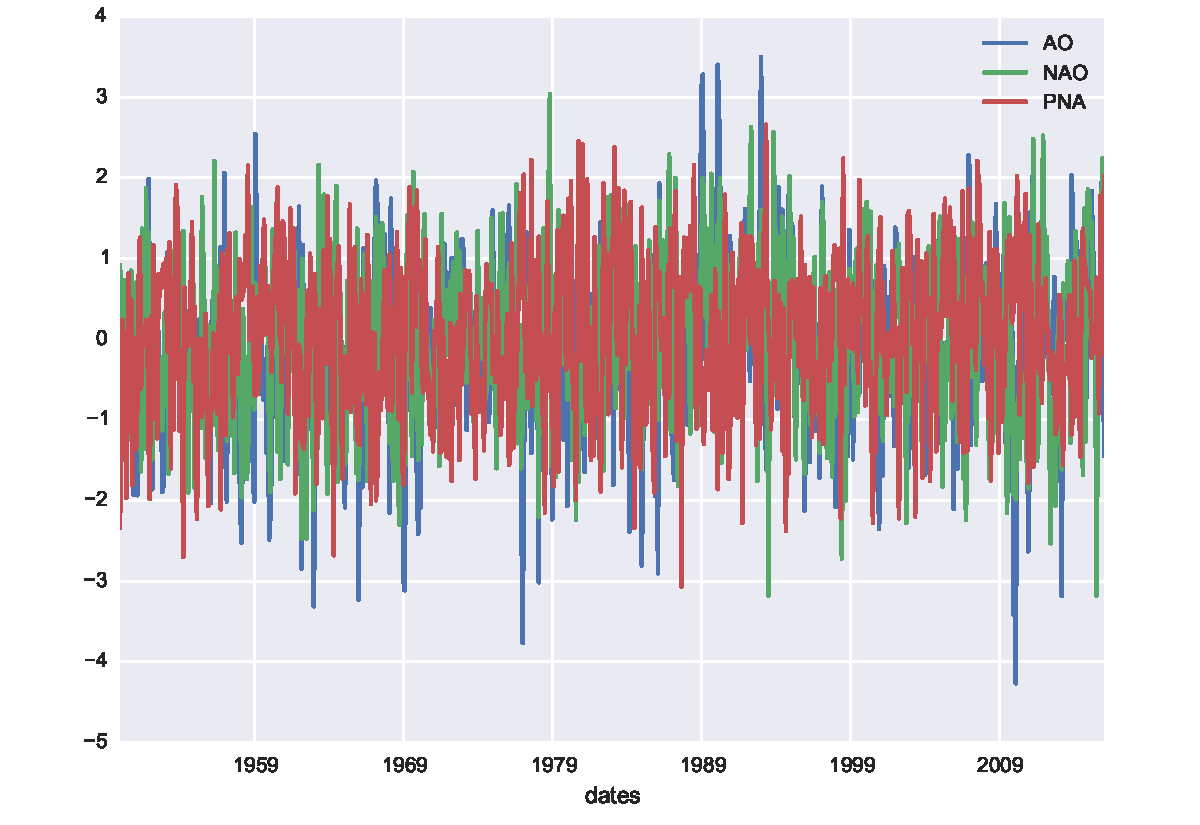
\includegraphics[width=0.8\linewidth]{./figs/fig1.pdf}
\caption{Time Series of AO (blue), NAO (green), and PNA (red) climate indices.}\label{fig:ts_idx}
\end{center}
\end{figure}

\begin{figure}
\begin{center}
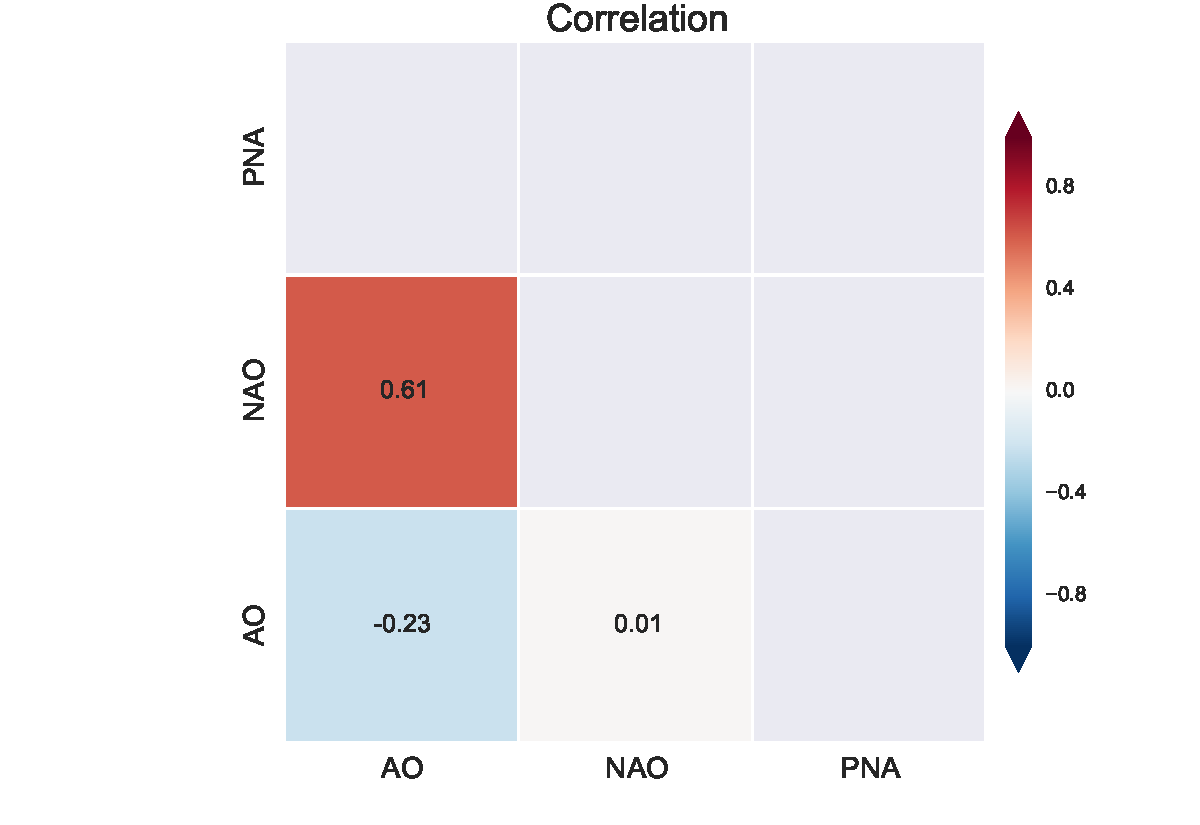
\includegraphics[width=0.8\linewidth]{./figs/fig2.pdf}
\caption{Correlation Matrix.}\label{fig:r_matrix}
\end{center}
\end{figure}

\newpage

\begin{figure}
\begin{center}
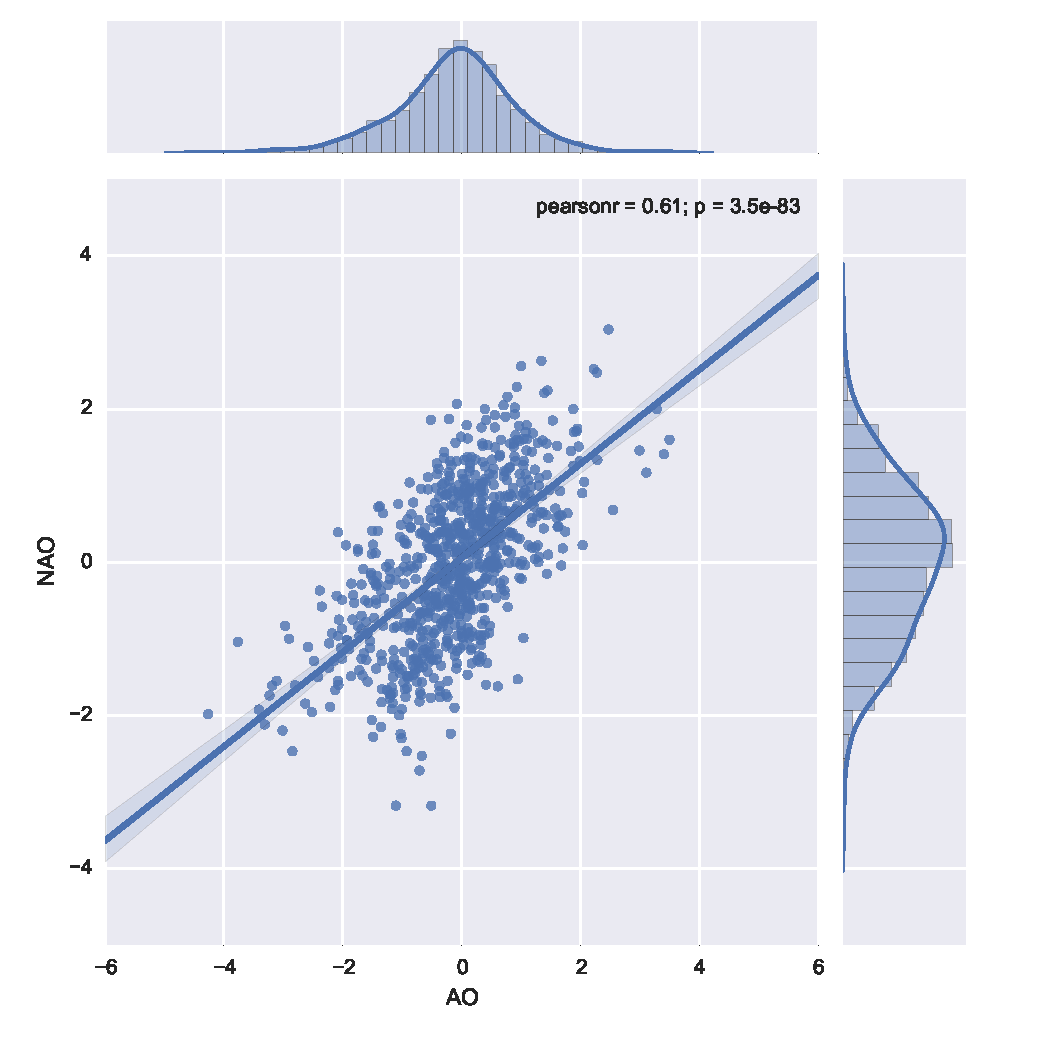
\includegraphics[width=0.8\linewidth]{./figs/fig3.pdf}
\caption{AO, NAO joint PDFs  and the linear regression fit.}\label{fig:joint_reg}
\end{center}
\end{figure}

\
\end{document}

%%%%%%%%%%%%%%%%%%%%%%%%%%%%%%%%%%%%%%%%%%%%%%%%%%%%%%%%%%%%%%%
